
%(BEGIN_QUESTION)
% Copyright 2011, Tony R. Kuphaldt, released under the Creative Commons Attribution License (v 1.0)
% This means you may do almost anything with this work of mine, so long as you give me proper credit

Two valves control the flow of air and fuel to the burner of a large furnace, shown in the following diagram.  The air valve is controlled by furnace temperature, and the fuel valve is controlled by the air flow so as to maintain a constant air/fuel ratio:

$$\includegraphics[width=15.5cm]{i01630x01.eps}$$

Choose the proper {\it fail-safe mode} for each valve so that the burner shuts down and all unburned fuel vapors in the furnace will be purged out the exhaust stack in the event of a general compressed air failure (i.e. both valves losing air pressure).

\vskip 10pt

Air valve must fail ({\it open} or {\it closed}?) \hskip 100pt Fuel valve must fail ({\it open} or {\it closed}?)

\vskip 10pt

Then, determine the proper control action for each controller (temperature controller -- TC ; and flow controller -- FC), assuming that both transmitters are direct-acting (greater temperature and greater flow = greater output signal to controller).

\vskip 10pt

Fuel flow controller action = {\it direct} or {\it reverse}?

\vskip 10pt

Temperature controller action = {\it direct} or {\it reverse}?

\underbar{file i01630}
%(END_QUESTION)





%(BEGIN_ANSWER)

{\it 2 points for each correct valve failure mode; 3 points for each correct controller action:}

\vskip 10pt

Air valve must fail \underbar{\bf open} \hskip 100pt Fuel valve must fail \underbar{\bf closed}

\vskip 10pt

Fuel flow controller action = {\bf reverse}

\vskip 10pt

Temperature controller action = {\bf direct}

%(END_ANSWER)





%(BEGIN_NOTES)

{\bf This question is intended for exams only and not worksheets!}.

%(END_NOTES)


